Com base no proposto por esse modelo, um programa de sistemas multiagentes é descrito por \textit{Agents} (agentes), \textit{Facts} (fatos), \textit{Effects} (efeitos), \textit(Count-as rules) (regras que determinam o adequado comportamento do agente), \textit{Sanction rules} (regras de sanção) \cite{dastaniframework}. 

Os \textit{Agents} são definidos em termos de duas \textit{strings} e um inteiro. A primeira \textit{string} é \textit{agentName} e é usado para definir o nome do agente e a segunda \textit{string} é \textit{agentProg} e define o nome  do arquivo onde se encontra especificações do respectivo agente. O inteiro \textit{nr} é usado para definir a quantia do agente \cite{dastaniframework}.

Os \textit{Facts} são compostos por conjuntos de literais denominados de \textit{bruteFacts}. Esses são fatos onde ocorre uma violação que desencadeia em uma dada sanção \cite{dastaniframework}. 

Os \textit{Effects} são compostos por \textit{effects}. Estes, por sua vez, são estruturados em termos de \textit{b-literals} (conjuntos que contem literais onde estes, por sua vez, representam um dado estado de mundo), e \textit{actionName} onde este, por sua vez, descreve ações que geram trasições de um estado de mundo para outro estado \cite{dastaniframework}. 

Os \textit{Count-as rules} são compostos por \textit{counts-as}. Esses, por sua vez, definem regras normativas. Isso implica em relações de implicabilidade que resultam em uma dada violação \cite{dastaniframework}. 

Os \textit{Sanction rules} são estruturados por \textit{sanctions}. Esses, por sua vez, definem regras de implicabilidade que competem a uma tratativa da violação \cite{dastaniframework}.
 
A figura a seguir ilustra um exemplo de um programa de sistema multiagente escrito nesta linguagem;


\begin{figure}[H]
  \centering
  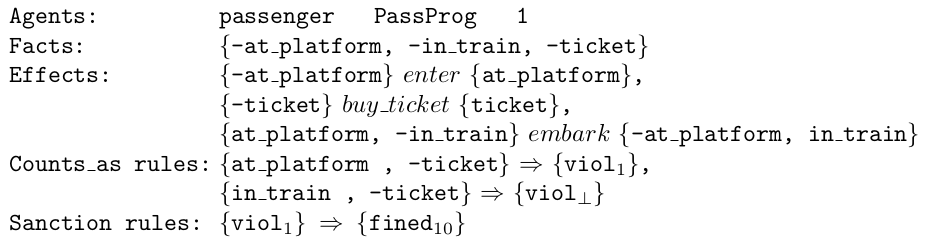
\includegraphics[width=0.8\linewidth]{figure/programdastani.png} 
  \caption{Um programa descrito na linguagem proposta neste estudo onde um agente representa um passageiro em uma estação de trem que pode entrar com ou sem um \textit{ticket} na plataforma e no trem \cite{dastaniframework}.}
  \label{exemploprograma}
\end{figure}


A figura \ref{exemploprograma} apresenta um programa que contem um agente com nome \textit{passenger}. O agente pode estar ou não na plataforma e no trem, sem ou com \textit{ticket}. Se o agente entrar na plataforma ou no trem sem o \textit{ticket}, então esse agente cometeu uma violação. Para este programa, a sanção da violação que ocorre por entrar na plataforma sem o \textit{ticket} resulta em uma punição onde o agente deve pagar 10 Euros pelo ocorrido \cite{dastaniframework}.
